\documentclass{article}

% Required packages (merged from hw5_template.tex and hw6_questions.tex)
\usepackage{amssymb}
\usepackage{amsmath}
\usepackage{graphicx}
\usepackage{geometry}
\usepackage{tikz}
\usepackage{array}
\usepackage{booktabs}
\usepackage{enumitem}
\usepackage{listings}
\usepackage{xcolor}
\usepackage{fancyhdr}
\usepackage{float}
\usepackage{subcaption}
\usepackage{comment}
\usepackage{algorithm}
\usepackage{algpseudocode}
\usepackage{caption}
\usepackage{siunitx}
\usepackage{hyperref}
\usetikzlibrary{arrows.meta, positioning} % Required for hw6 diagrams

% Set page geometry
\geometry{a4paper, margin=1in}

% Configure listings for Python
\lstset{
  language=Python,
  basicstyle=\ttfamily\footnotesize,
  numbers=left,
  numberstyle=\tiny\color{gray},
  frame=single,
  breaklines=true,
  breakatwhitespace=true,
  captionpos=b,
  tabsize=4,
  showspaces=false,
  showstringspaces=false,
  showtabs=false,
  commentstyle=\color{gray}\textit,
  keywordstyle=\color{blue}\bfseries,
  stringstyle=\color{red}
}

\begin{document}

\pagestyle{fancy}
\chead{DSC 257: Unsupervised Learning (Fall 2025)}
\lhead{Homework 6}
\rhead{Randall Rogers}

%------------------
% Solution for 1(a)
%------------------
\subsection*{Solution 1}
\noindent\rule{\textwidth}{0.4pt}\\
\subsubsection*{Question 1 (a)}
\begin{flushleft}
\textit{Experiments with the EM algorithm:} In this problem, we'll generate data from a mixture of Gaussians and then see whether the EM algorithm is able to recover the correct clustering and the correct parameters of the mixture model.
\end{flushleft}
\begin{flushleft}
    Consider a mixture of four Gaussians in $\mathbb{R}^2$ such that:
\end{flushleft}
$$p(x) = \pi_1 N(\mu_1, \Sigma_1) + \pi_2 N(\mu_2, \Sigma_2) + \pi_3 N(\mu_3, \Sigma_3) + \pi_4 N(\mu_4, \Sigma_4)$$
\begin{flushleft}
    where the mixing weights $\pi_i \ni i \in \{1,2,3,4\} \text{ and } \pi_i \in \mathbb{R}$ are given by:
\end{flushleft}
$$\pi_1 = 0.1, \pi_2 = 0.2, \pi_3 = 0.5, \pi_4 = 0.2$$
\begin{flushleft}
    the cluster means $\mu_i \in \mathbb{R}^2$ are given by:
\end{flushleft}
$$\mu_1 = \begin{bmatrix}7 \\ 6\end{bmatrix}, \mu_2 = \begin{bmatrix}0 \\ 0\end{bmatrix}, \mu_3 = \begin{bmatrix}-1 \\ 4\end{bmatrix}, \mu_4 = \begin{bmatrix}5 \\ -2\end{bmatrix}$$
\begin{flushleft}
    and the covariance matrices $\Sigma_i \in \mathbb{R}^{2 \times 2}$ are given by:
\end{flushleft}
$$\Sigma_1 = \begin{bmatrix}1 & 0 \\ 0 & 25\end{bmatrix}, \Sigma_2 = \begin{bmatrix}1 & 0 \\ 0 & 1\end{bmatrix}, \Sigma_3 = \begin{bmatrix}9 & 1 \\ 1 & 1\end{bmatrix}, \Sigma_4 = \begin{bmatrix}16 & -6 \\ -6 & 4\end{bmatrix}$$
\begin{itemize}
    \item Generate 400 points at random from this mixture model.
    \item Plot the points, using colors to distinguish the four components. Put this plot in your solution.
\end{itemize}
\subsubsection*{Solution 1 (a)}
\subsubsection*{Python Code}
\begin{lstlisting}
import numpy as np
import matplotlib.pyplot as plt

# set random seed
np.random(42)

# define mixture model parameters

# generate 400 random points from the mixture model

# plot points, using colors to distinguish each of the components
\end{lstlisting}

\subsubsection*{Plot}
\begin{comment}
\begin{figure}[h!]
\centering
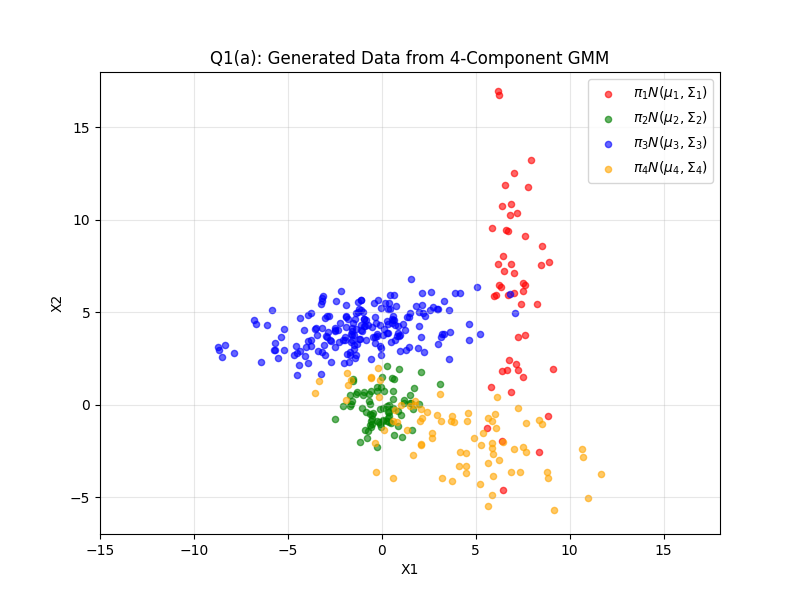
\includegraphics[width=0.7\textwidth]{q1a.png}
\caption{Visualization of the 400 random points generated from the mixture model.}
\label{fig:1a}
\end{figure}
\end{comment}

\subsubsection*{\normalfont}{$\therefore$ }

\subsubsection*{Graduate Level Explanation}

\subsubsection*{Learn Fast Explanation}

\noindent\rule{\textwidth}{0.4pt}\\

\newpage

%------------------
% Solution for 1(b)
%------------------
\subsection*{Solution 1}
\noindent\rule{\textwidth}{0.4pt}\\
\subsubsection*{Question 1 (b)}
\begin{flushleft}
\textit{Experiments with the EM algorithm:} In this problem, we'll generate data from a mixture of Gaussians and then see whether the EM algorithm is able to recover the correct clustering and the correct parameters of the mixture model.
\end{flushleft}
\begin{flushleft}
    Consider a mixture of four Gaussians in $\mathbb{R}^2$ such that:
\end{flushleft}
$$p(x) = \pi_1 N(\mu_1, \Sigma_1) + \pi_2 N(\mu_2, \Sigma_2) + \pi_3 N(\mu_3, \Sigma_3) + \pi_4 N(\mu_4, \Sigma_4)$$
\begin{flushleft}
    where the mixing weights $\pi_i \ni i \in \{1,2,3,4\} \text{ and } \pi_i \in \mathbb{R}$ are given by:
\end{flushleft}
$$\pi_1 = 0.1, \pi_2 = 0.2, \pi_3 = 0.5, \pi_4 = 0.2$$
\begin{flushleft}
    the cluster means $\mu_i \in \mathbb{R}^2$ are given by:
\end{flushleft}
$$\mu_1 = \begin{bmatrix}7 \\ 6\end{bmatrix}, \mu_2 = \begin{bmatrix}0 \\ 0\end{bmatrix}, \mu_3 = \begin{bmatrix}-1 \\ 4\end{bmatrix}, \mu_4 = \begin{bmatrix}5 \\ -2\end{bmatrix}$$
\begin{flushleft}
    and the covariance matrices $\Sigma_i \in \mathbb{R}^{2 \times 2}$ are given by:
\end{flushleft}
$$\Sigma_1 = \begin{bmatrix}1 & 0 \\ 0 & 25\end{bmatrix}, \Sigma_2 = \begin{bmatrix}1 & 0 \\ 0 & 1\end{bmatrix}, \Sigma_3 = \begin{bmatrix}9 & 1 \\ 1 & 1\end{bmatrix}, \Sigma_4 = \begin{bmatrix}16 & -6 \\ -6 & 4\end{bmatrix}$$
\begin{itemize}
    \item Write a routine that takes a two-dimensional Gaussian mixture (means and covariance matrices) and plots ellipses corresponding to each component. Using this routine, plot all the data points (from (a)) in the same color and then draw four ellipses on the same plot, depicting representative contours of the four Gaussians.
\end{itemize}
\subsubsection*{Solution 1 (b)}
\subsubsection*{Python Code}
\textit{NOTE: points from part(a) should be on same plot as ellipses}
\begin{lstlisting}

# from part(a)
import numpy as np
import matplotlib.pyplot as plt

# set random seed
np.random(42)
# define mixture model parameters

# generate 400 random points from the mixture model

# plot points, using colors to distinguish each of the components


# routine that takes 2D Gaussian mixture(mu_i,sigma_i) and plots ellipses coresponding to each component
from matplotlib.patches import Ellipse
eigvals, eigvecs = np.linalg.eigh(sigma)
direction = eigvecs[0] / np.linalg.norm(eigvecs[0])
theta = np.arctan2(direction[1], direction[0]) * 180 / np.pi + 180
stretch = 2.0 * np.sqrt(3.0 * eigvals)
ellipse = Ellipse(mu, stretch[0], stretch[1], angle=theta, color='red')
ellipse.set_alpha(0.25)
ax.add_artist(ellipse)

\end{lstlisting}

\subsubsection*{Plot}
\begin{comment}
\begin{figure}[h!]
\centering
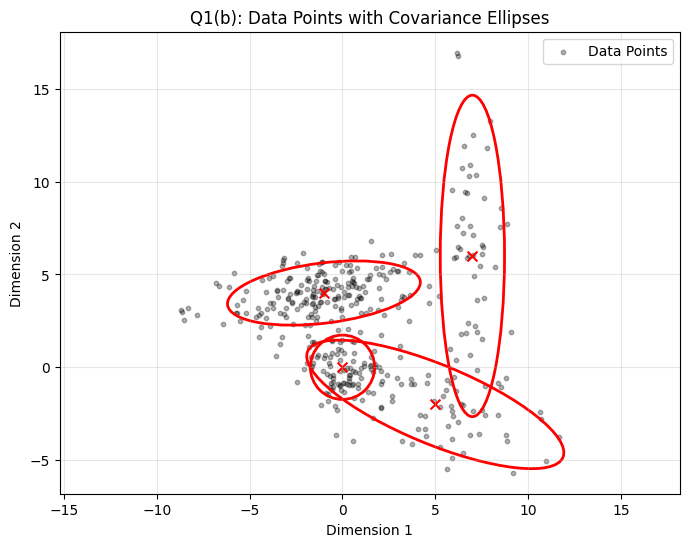
\includegraphics[width=0.7\textwidth]{q1b.png}
\caption{Visualization of the 400 random points generated from the mixture model with ellipses.}
\label{fig:1b}
\end{figure}
\end{comment}

\subsubsection*{\normalfont}{$\therefore$ }

\subsubsection*{Graduate Level Explanation}

\subsubsection*{Learn Fast Explanation}

\noindent\rule{\textwidth}{0.4pt}\\

\newpage

%------------------
% Solution for 1(c)
%------------------
\subsection*{Solution 1}
\noindent\rule{\textwidth}{0.4pt}\\
\subsubsection*{Question 1 (c)}
\begin{flushleft}
\textit{Experiments with the EM algorithm:} In this problem, we'll generate data from a mixture of Gaussians and then see whether the EM algorithm is able to recover the correct clustering and the correct parameters of the mixture model.
\end{flushleft}
\begin{flushleft}
    Consider a mixture of four Gaussians in $\mathbb{R}^2$ such that:
\end{flushleft}
$$p(x) = \pi_1 N(\mu_1, \Sigma_1) + \pi_2 N(\mu_2, \Sigma_2) + \pi_3 N(\mu_3, \Sigma_3) + \pi_4 N(\mu_4, \Sigma_4)$$
\begin{flushleft}
    where the mixing weights $\pi_i \ni i \in \{1,2,3,4\} \text{ and } \pi_i \in \mathbb{R}$ are given by:
\end{flushleft}
$$\pi_1 = 0.1, \pi_2 = 0.2, \pi_3 = 0.5, \pi_4 = 0.2$$
\begin{flushleft}
    the cluster means $\mu_i \in \mathbb{R}^2$ are given by:
\end{flushleft}
$$\mu_1 = \begin{bmatrix}7 \\ 6\end{bmatrix}, \mu_2 = \begin{bmatrix}0 \\ 0\end{bmatrix}, \mu_3 = \begin{bmatrix}-1 \\ 4\end{bmatrix}, \mu_4 = \begin{bmatrix}5 \\ -2\end{bmatrix}$$
\begin{flushleft}
    and the covariance matrices $\Sigma_i \in \mathbb{R}^{2 \times 2}$ are given by:
\end{flushleft}
$$\Sigma_1 = \begin{bmatrix}1 & 0 \\ 0 & 25\end{bmatrix}, \Sigma_2 = \begin{bmatrix}1 & 0 \\ 0 & 1\end{bmatrix}, \Sigma_3 = \begin{bmatrix}9 & 1 \\ 1 & 1\end{bmatrix}, \Sigma_4 = \begin{bmatrix}16 & -6 \\ -6 & 4\end{bmatrix}$$
\begin{itemize}
    \item Look at the plots from (a) and (b) and check that the shapes of the clusters correspond to what you would expect from the covariance matrices. One of the clusters is small and is partially contained within another cluster. Which clusters are these?
\end{itemize}
\subsubsection*{Solution 1 (c)}
\subsubsection*{Plot}
\begin{comment}
\begin{figure}[h!]
\centering
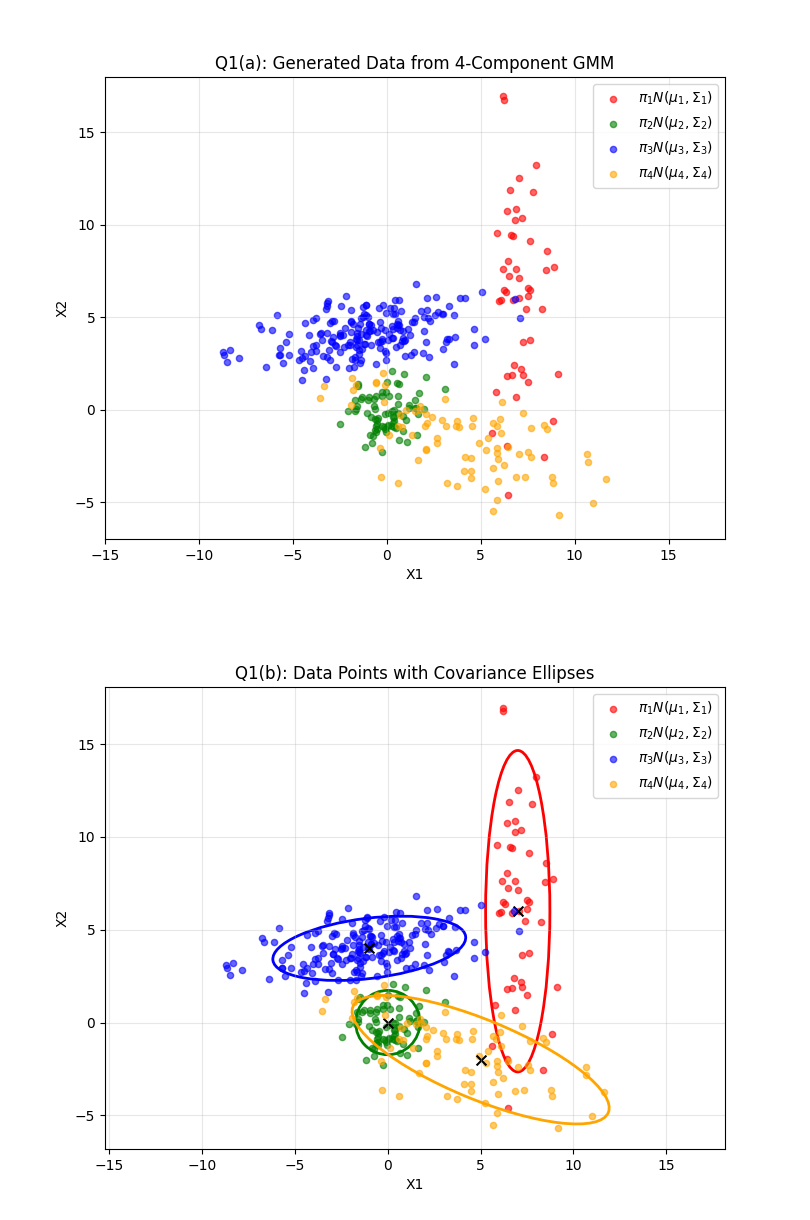
\includegraphics[width=0.7\textwidth]{q1c.png}
\caption{Comparision of plots from part (a) and (b)).}
\label{fig:q1c}
\end{figure}
\end{comment}

\subsubsection*{Plot Comparision Comments}
\begin{flushleft}
    \textit{One of the clusters is small and is partially contained within another cluster. Which clusters are these?}
\end{flushleft}


\subsubsection*{\normalfont}{$\therefore$ }

\subsubsection*{Graduate Level Explanation}

\subsubsection*{Learn Fast Explanation}

\noindent\rule{\textwidth}{0.4pt}\\

\newpage

%------------------
% Solution for 1(d)
%------------------
\subsection*{Solution 1}
\noindent\rule{\textwidth}{0.4pt}\\
\subsubsection*{Question 1 (d)}
\begin{flushleft}
\textit{Experiments with the EM algorithm:} In this problem, we'll generate data from a mixture of Gaussians and then see whether the EM algorithm is able to recover the correct clustering and the correct parameters of the mixture model.
\end{flushleft}
\begin{flushleft}
    Consider a mixture of four Gaussians in $\mathbb{R}^2$ such that:
\end{flushleft}
$$p(x) = \pi_1 N(\mu_1, \Sigma_1) + \pi_2 N(\mu_2, \Sigma_2) + \pi_3 N(\mu_3, \Sigma_3) + \pi_4 N(\mu_4, \Sigma_4)$$
\begin{flushleft}
    where the mixing weights $\pi_i \ni i \in \{1,2,3,4\} \text{ and } \pi_i \in \mathbb{R}$ are given by:
\end{flushleft}
$$\pi_1 = 0.1, \pi_2 = 0.2, \pi_3 = 0.5, \pi_4 = 0.2$$
\begin{flushleft}
    the cluster means $\mu_i \in \mathbb{R}^2$ are given by:
\end{flushleft}
$$\mu_1 = \begin{bmatrix}7 \\ 6\end{bmatrix}, \mu_2 = \begin{bmatrix}0 \\ 0\end{bmatrix}, \mu_3 = \begin{bmatrix}-1 \\ 4\end{bmatrix}, \mu_4 = \begin{bmatrix}5 \\ -2\end{bmatrix}$$
\begin{flushleft}
    and the covariance matrices $\Sigma_i \in \mathbb{R}^{2 \times 2}$ are given by:
\end{flushleft}
$$\Sigma_1 = \begin{bmatrix}1 & 0 \\ 0 & 25\end{bmatrix}, \Sigma_2 = \begin{bmatrix}1 & 0 \\ 0 & 1\end{bmatrix}, \Sigma_3 = \begin{bmatrix}9 & 1 \\ 1 & 1\end{bmatrix}, \Sigma_4 = \begin{bmatrix}16 & -6 \\ -6 & 4\end{bmatrix}$$
\begin{itemize}
    \item Now run the EM algorithm on the data. Plot the data, and using the procedure from (b), draw four ellipses on the same plot, depicting the four Gaussians returned by EM. How close are they to the correct Gaussians?
\end{itemize}
\subsubsection*{Solution 1 (d)}
\subsubsection*{Python Code}

\begin{lstlisting}
from sklearn.mixture import GaussianMixture

\end{lstlisting}

\subsubsection*{Plot}
\begin{comment}
\begin{figure}[h!]
\centering
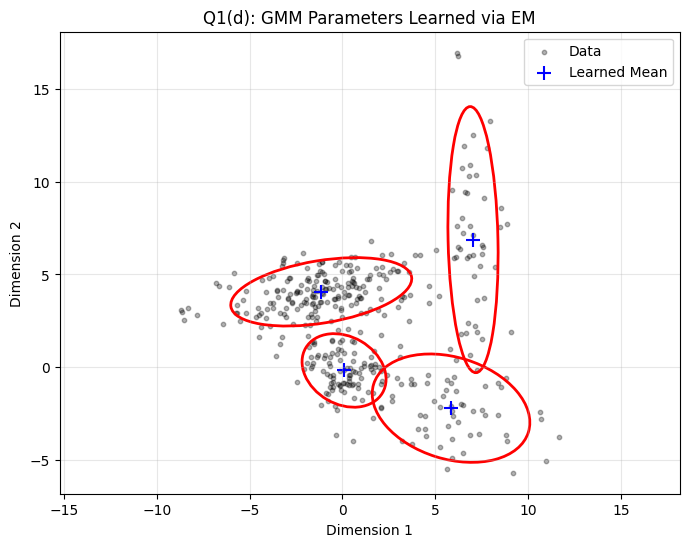
\includegraphics[width=0.7\textwidth]{q1d.png}
\caption{EM alorithim on data}
\label{fig:q1d}
\end{figure}
\end{comment}

\subsubsection*{Plot Comparision Comments}
\begin{flushleft}
    \textit{How close are they to the correct Gaussians?}
\end{flushleft}


\subsubsection*{\normalfont}{$\therefore$ }

\subsubsection*{Graduate Level Explanation}

\subsubsection*{Learn Fast Explanation}

\noindent\rule{\textwidth}{0.4pt}\\

\newpage

%------------------
% Solution for 1(e)
%------------------
\subsection*{Solution 1}
\noindent\rule{\textwidth}{0.4pt}\\
\subsubsection*{Question 1 (e)}
\begin{flushleft}
\textit{Experiments with the EM algorithm:} In this problem, we'll generate data from a mixture of Gaussians and then see whether the EM algorithm is able to recover the correct clustering and the correct parameters of the mixture model.
\end{flushleft}
\begin{flushleft}
    Consider a mixture of four Gaussians in $\mathbb{R}^2$ such that:
\end{flushleft}
$$p(x) = \pi_1 N(\mu_1, \Sigma_1) + \pi_2 N(\mu_2, \Sigma_2) + \pi_3 N(\mu_3, \Sigma_3) + \pi_4 N(\mu_4, \Sigma_4)$$
\begin{flushleft}
    where the mixing weights $\pi_i \ni i \in \{1,2,3,4\} \text{ and } \pi_i \in \mathbb{R}$ are given by:
\end{flushleft}
$$\pi_1 = 0.1, \pi_2 = 0.2, \pi_3 = 0.5, \pi_4 = 0.2$$
\begin{flushleft}
    the cluster means $\mu_i \in \mathbb{R}^2$ are given by:
\end{flushleft}
$$\mu_1 = \begin{bmatrix}7 \\ 6\end{bmatrix}, \mu_2 = \begin{bmatrix}0 \\ 0\end{bmatrix}, \mu_3 = \begin{bmatrix}-1 \\ 4\end{bmatrix}, \mu_4 = \begin{bmatrix}5 \\ -2\end{bmatrix}$$
\begin{flushleft}
    and the covariance matrices $\Sigma_i \in \mathbb{R}^{2 \times 2}$ are given by:
\end{flushleft}
$$\Sigma_1 = \begin{bmatrix}1 & 0 \\ 0 & 25\end{bmatrix}, \Sigma_2 = \begin{bmatrix}1 & 0 \\ 0 & 1\end{bmatrix}, \Sigma_3 = \begin{bmatrix}9 & 1 \\ 1 & 1\end{bmatrix}, \Sigma_4 = \begin{bmatrix}16 & -6 \\ -6 & 4\end{bmatrix}$$
\begin{itemize}
    \item Plot the data again, but this time color each point according to it most likely mixture component. How does this clustering compare to the true component memberships from \textit{part (a)}? Are dependencies understandable?
\end{itemize}
\subsubsection*{Solution 1 (e)}
\subsubsection*{Python Code}

\begin{lstlisting}
from sklearn.mixture import GaussianMixture

\end{lstlisting}

\subsubsection*{Plot}
\begin{comment}
\begin{figure}[h!]
\centering
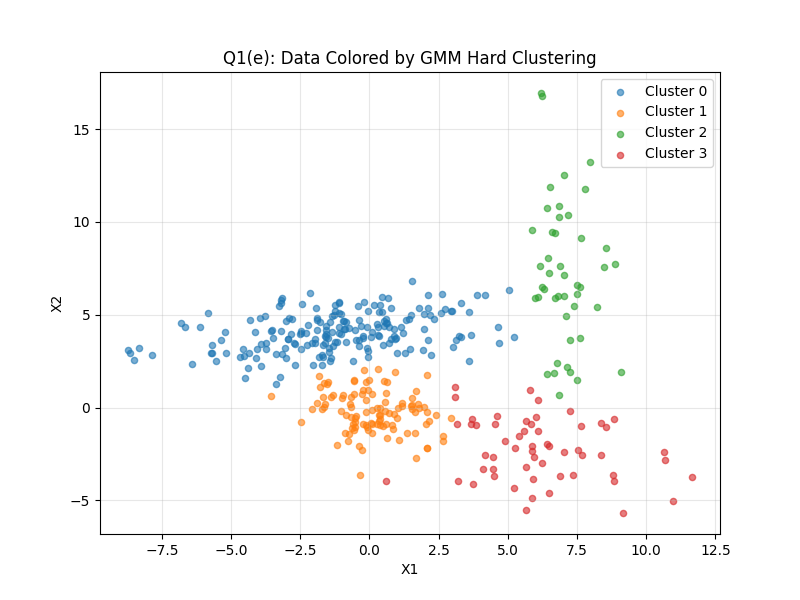
\includegraphics[width=0.7\textwidth]{q1e.png}
\caption{Color represents to it's most likeyly mixture component}
\label{fig:q1e}
\end{figure}
\end{comment}

\subsubsection*{Plot Comments}
\begin{flushleft}
    \textit{How does this clustering compare to the true component memberships (from (a))?}
\end{flushleft}
\begin{flushleft}
    \textit{Are the discrepancies understandable?}
\end{flushleft}


\subsubsection*{\normalfont}{$\therefore$ }

\subsubsection*{Graduate Level Explanation}

\subsubsection*{Learn Fast Explanation}

\noindent\rule{\textwidth}{0.4pt}\\

\newpage

%------------------
% Solution for 1(f)
%------------------
\subsection*{Solution 1}
\noindent\rule{\textwidth}{0.4pt}\\
\subsubsection*{Question 1 (f)}
\begin{flushleft}
\textit{Experiments with the EM algorithm:} In this problem, we'll generate data from a mixture of Gaussians and then see whether the EM algorithm is able to recover the correct clustering and the correct parameters of the mixture model.
\end{flushleft}
\begin{flushleft}
    Consider a mixture of four Gaussians in $\mathbb{R}^2$ such that:
\end{flushleft}
$$p(x) = \pi_1 N(\mu_1, \Sigma_1) + \pi_2 N(\mu_2, \Sigma_2) + \pi_3 N(\mu_3, \Sigma_3) + \pi_4 N(\mu_4, \Sigma_4)$$
\begin{flushleft}
    where the mixing weights $\pi_i \ni i \in \{1,2,3,4\} \text{ and } \pi_i \in \mathbb{R}$ are given by:
\end{flushleft}
$$\pi_1 = 0.1, \pi_2 = 0.2, \pi_3 = 0.5, \pi_4 = 0.2$$
\begin{flushleft}
    the cluster means $\mu_i \in \mathbb{R}^2$ are given by:
\end{flushleft}
$$\mu_1 = \begin{bmatrix}7 \\ 6\end{bmatrix}, \mu_2 = \begin{bmatrix}0 \\ 0\end{bmatrix}, \mu_3 = \begin{bmatrix}-1 \\ 4\end{bmatrix}, \mu_4 = \begin{bmatrix}5 \\ -2\end{bmatrix}$$
\begin{flushleft}
    and the covariance matrices $\Sigma_i \in \mathbb{R}^{2 \times 2}$ are given by:
\end{flushleft}
$$\Sigma_1 = \begin{bmatrix}1 & 0 \\ 0 & 25\end{bmatrix}, \Sigma_2 = \begin{bmatrix}1 & 0 \\ 0 & 1\end{bmatrix}, \Sigma_3 = \begin{bmatrix}9 & 1 \\ 1 & 1\end{bmatrix}, \Sigma_4 = \begin{bmatrix}16 & -6 \\ -6 & 4\end{bmatrix}$$
\begin{itemize}
    \item Finally, let's see how EM's solution evolves over iterations of local search. Show four plots, depicting the progress of EM at different iterations.
\end{itemize}
\subsubsection*{Solution 1 (f)}
\subsubsection*{Python Code}

\begin{lstlisting}
from sklearn.mixture import GaussianMixture

\end{lstlisting}

\subsubsection*{Plot}
\begin{comment}
\begin{figure}[h!]
\centering
\includegraphics[width=0.7\textwidth]{q1f_1.png}
\caption{Itteration 1 of EM algorithm on data}
\label{fig:q1f_1}
\end{figure}
\end{comment}

\begin{comment}
\begin{figure}[h!]
\centering
\includegraphics[width=0.7\textwidth]{q1f_10.png}
\caption{Itteration 10 of EM algorithm on data}
\label{fig:q1f_10}
\end{figure}
\end{comment}

\begin{comment}
\begin{figure}[h!]
\centering
\includegraphics[width=0.7\textwidth]{q1f_50.png}
\caption{Itteration 50 of EM algorithm on data}
\label{fig:q1f}
\end{figure}
\end{comment}




\subsubsection*{\normalfont}{$\therefore$ }

\subsubsection*{Graduate Level Explanation}

\subsubsection*{Learn Fast Explanation}

\noindent\rule{\textwidth}{0.4pt}\\

\newpage


%------------------
% Solution for 2(a)
%------------------
\subsection*{Solution 2}
\noindent\rule{\textwidth}{0.4pt}\\
\subsubsection*{Question 2 (a)}
\begin{flushleft}
\textit{Kernel density estimation:} Suppose we have samples $x_1, x_2, \ldots, x_n \in \mathbb{R}^d$ from an unknown distribution $f$, and we want to come up with a model of $f$. One simple way to do this is using the kernel density estimator $\widehat{f}$, which approximates $f$ using a mixture of $n$ Gaussians, each with weight $1/n$, and each centered at one of the data points:
\end{flushleft}
$$\widehat{f}: \frac{1}{n} N(x_1, \sigma^2 I_d) + \frac{1}{n} N(x_2, \sigma^2 I_d) + \cdots + \frac{1}{n} N(x_n, \sigma^2 I_d)$$
\begin{flushleft}
    Here $\sigma$ must be selected carefully. It is usually called the bandwidth parameter.
\end{flushleft}
\begin{figure}[h!]
\centering
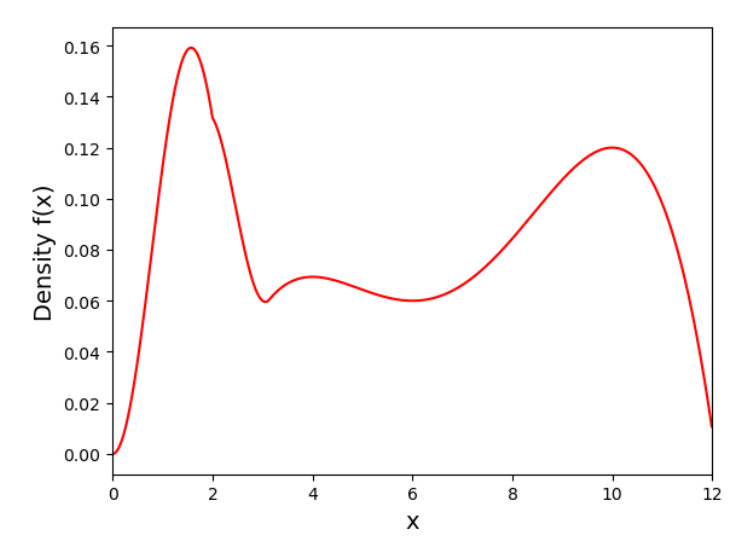
\includegraphics[width=0.7\textwidth]{q2.png}
\caption{The file \texttt{samples.txt} contains 1,000 samples drawn from $f$ (using rejection sampling).}
\label{fig:q2}
\end{figure}
\begin{itemize}
    \item Plot a histogram of the 1,000 samples using 20 bins.It should (very roughly) resemble the distribution f shown above.
\end{itemize}
\subsubsection*{Solution 2 (a)}
\subsubsection*{Python Code}

\begin{lstlisting}
import matplotlib.pyplot as plt

\end{lstlisting}

\subsubsection*{Plot}
\begin{comment}
\begin{figure}[h!]
\centering
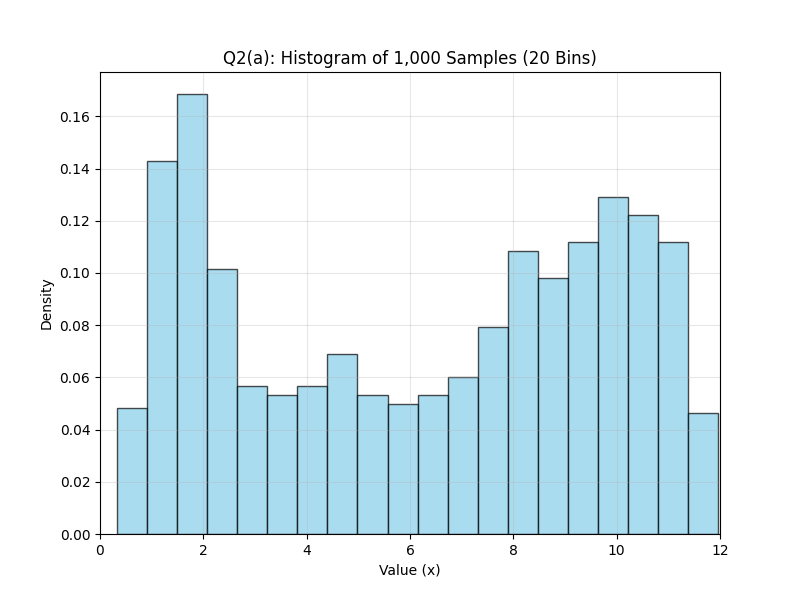
\includegraphics[width=0.7\textwidth]{q2a.png}
\caption{Histogram of 1,000 samples using 20 bins}
\label{fig:q2a}
\end{figure}
\end{comment}


\subsubsection*{\normalfont}{$\therefore$ }

\subsubsection*{Graduate Level Explanation}

\subsubsection*{Learn Fast Explanation}

\noindent\rule{\textwidth}{0.4pt}\\

\newpage

%------------------
% Solution for 2(b)
%------------------
\subsection*{Solution 2}
\noindent\rule{\textwidth}{0.4pt}\\
\subsubsection*{Question 2 (b)}
\begin{flushleft}
\textit{Kernel density estimation:} Suppose we have samples $x_1, x_2, \ldots, x_n \in \mathbb{R}^d$ from an unknown distribution $f$, and we want to come up with a model of $f$. One simple way to do this is using the kernel density estimator $\widehat{f}$, which approximates $f$ using a mixture of $n$ Gaussians, each with weight $1/n$, and each centered at one of the data points:
\end{flushleft}
$$\widehat{f}: \frac{1}{n} N(x_1, \sigma^2 I_d) + \frac{1}{n} N(x_2, \sigma^2 I_d) + \cdots + \frac{1}{n} N(x_n, \sigma^2 I_d)$$
\begin{flushleft}
    Here $\sigma$ must be selected carefully. It is usually called the bandwidth parameter.
\end{flushleft}
\begin{figure}[h!]
\centering
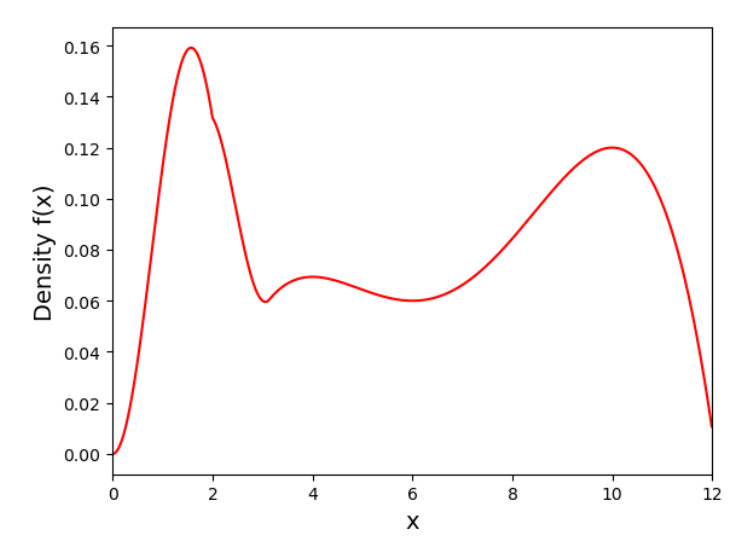
\includegraphics[width=0.7\textwidth]{q2.png}
\caption{The file \texttt{samples.txt} contains 1,000 samples drawn from $f$ (using rejection sampling).}
\end{figure}
\begin{itemize}
    \item Now apply kernel density estimation using just the first 100 samples in \texttt{samples.txt}, that is, $n=100$. For the bandwidth parameter, try the following settings: $0.25, 0.5, 0.75, 1.0$.
    \begin{itemize}
        \item For each of the four bandwidth settings, show a plot of the resulting density $\widehat{f}$.
        \item What changes as the bandwidth increases? Give a one- or two-sentence description.
        \item In this case, which of the four bandwidth settings yields a model $\widehat{f}$ that is closest to the original $f$, in your opinion?
    \end{itemize}
\end{itemize}
\subsubsection*{Solution 2 (b)}
\subsubsection*{Python Code}

\begin{lstlisting}
from sklearn.neighbors import KernelDensity
from matplotlib.pyplot as plt
from scipy.stats import norm
import numpy as np  

# define density settings
densities = [0.25,0.50,0.75,1.0]

\end{lstlisting}

\subsubsection*{Plot}
\begin{comment}
\begin{figure}[h!]
\centering
\includegraphics[width=0.7\textwidth]{q2b_1.png}
\caption{Bandwidth setting 1 (0.25)}
\label{fig:q2b_1}
\end{figure}
\end{comment}
\begin{comment}
\begin{figure}[h!]
\centering
\includegraphics[width=0.7\textwidth]{q2b_2.png}
\caption{Bandwidth setting 2(0.5)}
\label{fig:q2b_2}
\end{figure}
\end{comment}
\begin{comment}
\begin{figure}[h!]
\centering
\includegraphics[width=0.7\textwidth]{q2b_3.png}
\caption{Bandwidth setting 1 (0.75)}
\label{fig:q2b_3}
\end{figure}
\end{comment}
\begin{comment}
\begin{figure}[h!]
\centering
\includegraphics[width=0.7\textwidth]{q2b_4.png}
\caption{Bandwidth setting 2(1.0)}
\label{fig:q2b_4}
\end{figure}
\end{comment}

\subsubsection*{Plot Comments}
\textit{What changes as the bandwidth increases?}
\textit{Which bandwidth setting yeilds a model $\widehat{f}$ that is closest to the original $f$, in your opinion?}
\subsubsection*{\normalfont}{$\therefore$ }

\subsubsection*{Graduate Level Explanation}

\subsubsection*{Learn Fast Explanation}

\noindent\rule{\textwidth}{0.4pt}\\

\newpage

%------------------
% Solution for 2(c)
%------------------
\subsection*{Solution 2}
\noindent\rule{\textwidth}{0.4pt}\\
\subsubsection*{Question 2 (c)}
\begin{flushleft}
\textit{Kernel density estimation:} Suppose we have samples $x_1, x_2, \ldots, x_n \in \mathbb{R}^d$ from an unknown distribution $f$, and we want to come up with a model of $f$. One simple way to do this is using the kernel density estimator $\widehat{f}$, which approximates $f$ using a mixture of $n$ Gaussians, each with weight $1/n$, and each centered at one of the data points:
\end{flushleft}
$$\widehat{f}: \frac{1}{n} N(x_1, \sigma^2 I_d) + \frac{1}{n} N(x_2, \sigma^2 I_d) + \cdots + \frac{1}{n} N(x_n, \sigma^2 I_d)$$
\begin{flushleft}
    Here $\sigma$ must be selected carefully. It is usually called the bandwidth parameter.
\end{flushleft}
\begin{figure}[h!]
\centering
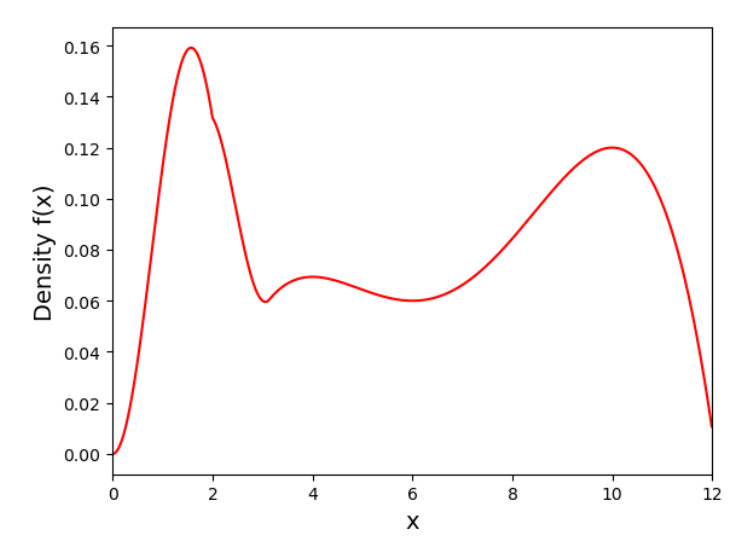
\includegraphics[width=0.7\textwidth]{q2.png}
\caption{The file \texttt{samples.txt} contains 1,000 samples drawn from $f$ (using rejection sampling).}
\end{figure}
\begin{itemize}
    \item Now show the plots of the kernel density estimate using all 1000 samples in \texttt{samples.txt}, that is, $n=1000$. Use the same four settings of the bandwidth.
\end{itemize}
\subsubsection*{Solution 2 (c)}
\subsubsection*{Python Code}

\begin{lstlisting}
from sklearn.neighbors import KernelDensity
from matplotlib.pyplot as plt
from scipy.stats import norm
import numpy as np  

# define density settings
densities = [0.25,0.50,0.75,1.0]

\end{lstlisting}

\subsubsection*{Plot}
\begin{comment}
\begin{figure}[h!]
\centering
\includegraphics[width=0.7\textwidth]{q2c_1.png}
\caption{Bandwidth setting 1 (0.25) for all 1000 samples}
\label{fig:q2c_1}
\end{figure}
\end{comment}
\begin{comment}
\begin{figure}[h!]
\centering
\includegraphics[width=0.7\textwidth]{q2c_2.png}
\caption{Bandwidth setting 2(0.5) for all 1000 samples}
\label{fig:q2c_2}
\end{figure}
\end{comment}
\begin{comment}
\begin{figure}[h!]
\centering
\includegraphics[width=0.7\textwidth]{q2c_3.png}
\caption{Bandwidth setting 1 (0.75) for all 1000 samples}
\label{fig:q2c_3}
\end{figure}
\end{comment}
\begin{comment}
\begin{figure}[h!]
\centering
\includegraphics[width=0.7\textwidth]{q2c_4.png}
\caption{Bandwidth setting 2(1.0) for all 1000 samples}
\label{fig:q2c_4}
\end{figure}
\end{comment}

\subsubsection*{\normalfont}{$\therefore$ }

\subsubsection*{Graduate Level Explanation}

\subsubsection*{Learn Fast Explanation}

\noindent\rule{\textwidth}{0.4pt}\\

\newpage

\end{document}
